\documentclass{standalone}
\usepackage{tikz}
  \usetikzlibrary{math}
\begin{document}

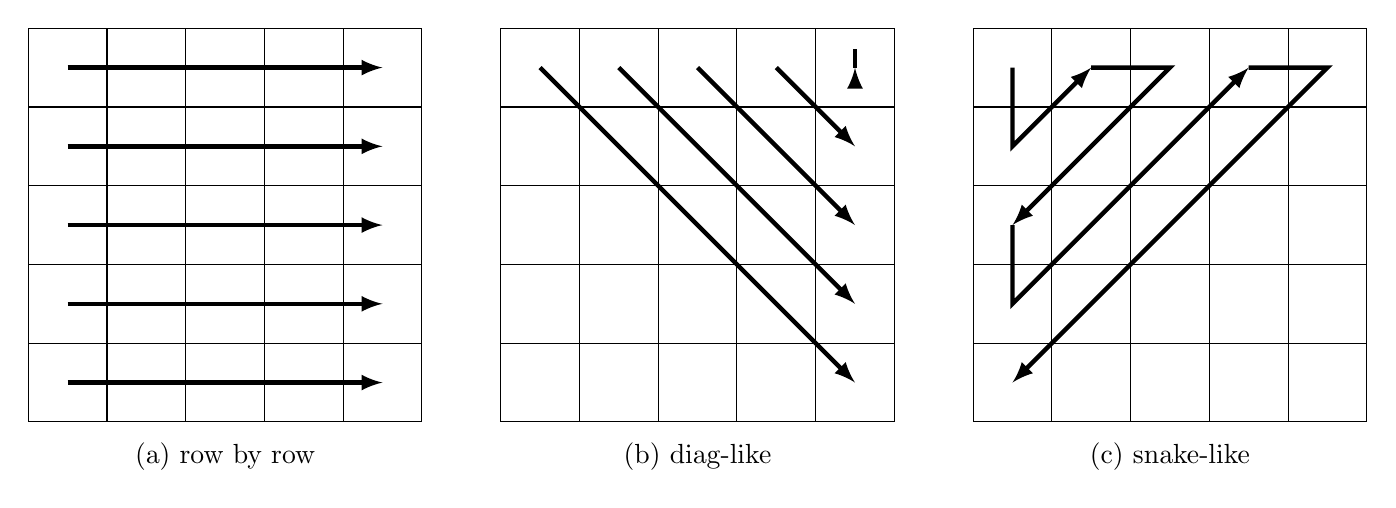
\begin{tikzpicture}
\tikzmath{\L=5;}
\tikzset{build/.style={-latex, ultra thick}}
\foreach \s in {0,6cm,12cm}
  \draw[xshift=\s] (0,0) grid (\L,\L);
% Row-by-row
\foreach \r in {1,...,\L}
  \draw[build] (.5,\r-.5) -- (\L-.5,\r-.5);
% Diag-like
\foreach \r in {1,...,\L}
  \draw[build, xshift=6cm] (\r-.5,\L-.5) -- (\L-.5,\r-.5);
% Snake-like
\foreach \s [count=\i] in {1,...,\L} {
  \pgfmathisodd{\i} 
  \ifnum\pgfmathresult>0 {
    \draw[build, xshift=12cm] (.5,\L-\s+.5) -- (.5,\L-\s-.5) -- (\s+.5,\L-.5);
  } \else {
    \draw[build, xshift=12cm] (\s-.5,\L-.5) -- (\s+.5,\L-.5) -- (.5,\L-\i-.5);
  } \fi
  \ifnum \i>3
    \breakforeach
  \fi
}
% Text
\foreach \s/\t in {0/{(a) row by row},6/{(b) diag-like},12/{(c) snake-like}}
  \node[below=4pt] at (2.5+\s,0) {\t};
\end{tikzpicture}

\end{document}